\chapter{Estado del arte del perfilado de autor}
\label{chap:estadoarte}

\lettrine{D}{urante} los inicios del perfilado automático de autor, los algoritmos se centraban en la tarea de la clasificación por género.
En esta línea, trabajos como Koppel et al., 2002 \cite{koppel2002automatically} se desmarcaban de la tendencia de la época,
la cual se basaba en la clasificación de textos en base a su contenido, para enfocarse en la clasificación de textos en base a su estilo.
En este caso, se centraban en la obtención del género del autor mediante el análisis
de 920 documentos de carácter formal escritos en inglés con una media de alrededor de 34.300 palabras cada uno, obteniendo una precisión en la clasificación de
aproximadamente el 77\%.

\bigskip
Así, la demostración de la existencia de rasgos diferenciadores en la escritura que permitían perfilar ciertos aspectos del individuo, especialmente del género,
supuso un gran avance en el campo del perfilado de autor
y dio pie a la realización de trabajos como Argamon et al., 2003 \cite{argamon2003gender}, Corney et al., 2002 \cite{corney2002gender} u Otterbacher et al., 2010 \cite{otterbacher2010inferring}.
Además, este hecho también permitió el inicio de una clasificación más compleja en base a otras características demográficas.

\bigskip
Posteriormente, tal como recoge Wiegmann et al., 2019 \cite{wiegmann2019overview}, se continuarían llevando a cabo estudios en esta línea, diversificando
las características a clasificar. En este sentido, se realizarían trabajos como Álvarez-Carmona et al., 2018 \cite{alvarez2018overview}, donde se buscaba
predecir el lugar de residencia del autor junto a su ocupación; otros como Volkova et al., 2015 \cite{volkova2015predicting}, en el que se trataba de perfilar la orientación política,
el salario, el optimismo del autor o su sentimiento de satisfacción vital; Preoţiuc-Pietro et al., 2018 \cite{preoctiuc2018user}, en el que se llevaba a cabo la tarea de
clasificar la raza y la etnia del autor; u otros como Fatima et al., 2017 \cite{fatima2017multilingual} que buscaban extender el perfilado de autor a otros idiomas. Asimismo,
la mayor parte de los \textit{datasets} utilizados para la creación de los modelos con estos algoritmos, se basaban en textos de redes sociales como Twitter (Burger et al., 2011) \cite{burger2011discriminating},
Facebook (Fatima et al., 2017) \cite{fatima2017multilingual} o Reddit (Gjurković et al., 2018) \cite{gjurkovic2018reddit}, reflejando así la importancia de estas plataformas
en la actualidad.

\bigskip
Por otro lado, en el año 2011, se celebraría el primer evento organizado por el \textit{PAN} (\textit{Plagiarism Analysis, Authorship Identification, and Near-Duplicate Detection}) \cite{pan},
uno de los foros de investigación más importantes que organiza eventos científicos y tareas anuales relacionadas con el análisis forense de textos digitales
y rasgos estilométricos, así como uno de los grandes implusores del perfilado de autor. La primera de las tareas centradas en este campo se celebraría en el año 2013 (Rangel et al., 2013) \cite{rangel2013overview},
en la que se pedía a los participantes que obtuvieran, a partir de una serie de \textit{tweets}, la edad y el género de su autor. El ganador de este concurso obtuvo una
precisión del 60\% en la clasificación de género y del 67\% en la clasificación de edad, haciendo uso, la mayor parte de los participantes, de técnicas de aprendizaje
supervisado como los Árboles de Decisión (\textit{Decission Trees} en inglés) o las Máquinas de Soporte Vectorial (\textit{Support Vector Machines} o SVMs en inglés).
Además, la mayoría de ellos incluyeron en sus modelos características basadas en el TF-IDF, n-gramas o etiquetas POS, explicadas en detalle en la Sección \ref{sec:conceptos_basicos},
junto a otras como el número de emoticonos o la frecuencia de signos de puntuación.
En los siguientes años se celebrarían nuevas ediciones con el perfilado de autor en el centro (Rangel et al., 2014 \cite{rangel2014overview}; Rangel et al., 2015 \cite{rangel2015overview};
Rangel et al., 2016 \cite{rangel2016overview}...), en las que se añadirían nuevas subtareas como el reconocimiento de rasgos personales, la ocupación o los dialectos del lenguaje,
así como también alcanzando mejores resultados en la clasificación.

\section{Conceptos básicos}
\label{sec:conceptos_basicos}

Cuando hablamos del perfilado automático de autores, nos referimos a la tarea del análisis detallado de un texto para la obtención de ciertas características
que nos permitan identificar a su autor.
Dicha tarea de análisis está enmarcada dentro del campo del procesado del lenguaje natural y, más concretamente,
dentro de la rama de la estilometría. De esta forma, para las tareas de NLP se hace uso
de una serie de algoritmos y técnicas que permiten la extracción de características formales de un texto que puedan
ser procesadas por un ordenador. Las más utilizadas y relevantes
para la comprensión de los análisis posteriores y, en general, de este trabajo son las siguientes:

\subsection{TF-IDF}
El TF-IDF (del inglés \textit{Term Frequency-Inverse Document Frequency}) es una medida estadística muy utilizada en el campo de la recuperación de información
(en inglés \textit{Information Retrieval} o IR) que expresa cuán relevante es una palabra para un documento en una colección.

\bigskip
El cálculo de dicha medida para cada palabra sigue la siguiente fórmula:

\begin{equation}
	\label{eq:tfidf}
	\text{TF-IDF}(t,d) = \text{TF}(t,d) \times \text{IDF}(t)
\end{equation}

Donde:
\begin{itemize}
	\item $t$ es la palabra de la que se quiere calcular el TF-IDF.
	\item $d$ es el documento en el que se encuentra la palabra.
	\item $\text{TF}(t,d)$ es la frecuencia de la palabra $t$ en el documento $d$, que se calcula como:
	      \begin{equation}
		      \label{eq:tf}
		      TF(t,d) = \frac{n_{t,d}}{n_d}
	      \end{equation}

	      Donde:
	      \begin{itemize}
		      \item $n_{t,d}$ es el número de veces que la palabra $t$ aparece en el documento $d$.
		      \item $n_d$ es el número total de palabras en el documento $d$.
	      \end{itemize}

	\item $\text{IDF}(t)$ es la frecuencia inversa de documentos que representa la importancia de la palabra $t$ en la colección de documentos y
	      se calcula como:
	      \begin{equation}
		      \label{eq:idf}
		      \text{IDF}(t) = \log \left(\frac{N}{\text{DF}(t)}\right)
	      \end{equation}

	      Donde:
	      \begin{itemize}
		      \item $N$ es el número total de documentos en la colección.
		      \item $\text{DF}(t)$ es el número de documentos en los que aparece la palabra $t$.
	      \end{itemize}
\end{itemize}

\bigskip
Por lo tanto, la importancia aumenta proporcionalmente al número de veces que una palabra aparece en el documento, pero se compensa con la frecuencia
de la palabra en la colección, lo que permite manejar el hecho de que algunas palabras son generalmente más comunes que otras.

\subsection{Etiquetas POS}

Las etiquetas POS (\textit{Part-Of-Speech} en inglés) son etiquetas gramaticales que se asignan a las palabras de un texto según su función sintáctica, es
decir, si se trata de un sustantivo, un verbo, un adjetivo, etc.
Existen varios tipos de etiquetas POS, pero las más empleadas son las descritas en el \textit{Penn Treebank Project} \cite{marcus1993building}.

\subsection{N-gramas}

Los n-gramas son una técnica de modelado de lenguaje que consiste en la extracción de secuencias de $n$ elementos de un texto. Estos elementos pueden ser de varios
tipos, entre ellos, caracteres, palabras o etiquetas POS. Las longitudes de dichas secuencias de elementos más habituales suelen oscilar entre uno y cuatro, dando como resultado los unigramas, bigramas,
trigramas y tetragramas.
Asimismo, los n-gramas suelen combinarse con el TF-IDF para proporcionar vectores de características que puedan ser utilizados por los algoritmos de clasificación.
Cabe destacar también que el TF-IDF, en su versión más común, es un caso particular de uso de los n-gramas, en concreto, de unigramas de palabras.

\subsection{\textit{Bag-of-words}}
\label{sec:bag_of_words}

La \textit{bag-of-words} o BoW es una técnica simple de representación de documentos que consiste en la extracción de las palabras que aparecen en un texto,
sin tener en cuenta el orden en el que aparecen ni la estructura gramatical de la que forman parte. De esta modo, se obtiene un vector de características en el
que cada posición representa una palabra y que tiene como valores el número de veces que aparece dicha palabra en el documento.

\subsection{Análisis Semántico Latente}
\label{sec:analisis_semantico_latente}

El Análisis Semántico Latente (\textit{Latent Semantic Analysis} o LSA en inglés) es una técnica de IR (del inglés \textit{Information Retrieval}) desarrollada por Deerwester et al., 1990 \cite{deerwester1990indexing}
que busca descubrir relaciones latentes
entre las palabras y los documentos que forman una colección. Esta técnica se basa
en el idea de que las palabras que aparecen en contextos similares
tienden a tener significados similares. Para aplicarla, se construye una matriz en la que se almacena la frecuencia de cada palabra del vocabulario en cada documento y
a continuación, se aplica una descomposición en valores singulares (\textit{Singular Value Decomposition} o SVD en inglés) a dicha matriz para reducir su dimensionalidad
y encontrar relaciones palabras-documentos.

\bigskip
Esta técnica tiene limitaciones, sobre todo a la hora de manejar sinónimos y polisemias, ya que al basarse únicamente en patrones estadísticos,
no tiene en cuenta el significado real de las palabras.

\section{Competiciones analizadas}
\label{sec:competiciones_analizadas}

Una vez explicados los conceptos básicos, procederemos en esta sección al análisis de las competiciones más relevantes en el contexto
del perfilado automático de autores. En este sentido, cabe destacar que, dado que el objetivo de este trabajo estaba encuadrado en
la investigación sobre algoritmos de perfilado de autores de habla inglesa, se obviaron otras competiciones relevantes como pueden ser
las organizadas por IberLEF \cite{iberlef}, un foro de investigación que promueve el desarrollo de sistemas basados en NLP en español y otras
lenguas ibéricas.
Asimismo, puesto que el perfilado de la edad era otra característica fundamental que debía incluir este trabajo, se seleccionaron aquellas competiciones
que contaban con dicha tarea, en este caso, las celebradas en los años 2014 (Rangel et al.) \cite{rangel2014overview}, 2015 (Rangel et al.) \cite{rangel2015overview} y 2019 (Wiegmann et al.) \cite{wiegmann2019overview}
por PAN.

\subsection{\textit{PAN Author Profiling 2014}}

Esta segunda edición de la competición internacional de perfilado de autores celebrada en 2014 por PAN, estaba enfocada en la clasificación de género y edad de los autores, en la que se consideraban, para esta última, las siguientes
clases: \textit{18-24}, \textit{25-34}, \textit{35-49}, \textit{50-64} y \textit{65-XX}; donde esta úlitma representa cualquier edad igual o superior a 65 años.

\subsubsection{\textit{Corpus}}

En lo referente al \textit{dataset} de entrenamiento y evaluación utilizado, la organización de la
competición elaboró un \textit{corpus} con documentos de diferentes tipos que incluían: \textit{tweets}, \textit{posts} de blogs, \textit{posts} de otras redes sociales y \textit{reviews} de hoteles.
Todos ellos contenían documentos en inglés y en español a excepción de las \textit{reviews} de hoteles, las cuales solo estaban disponibles en inglés.

\bigskip
Como se puede observar en la distribución de los autores, disponible tanto en la Tabla \ref{tab:dataset_2014} como en la Figura \ref{fig:dataset_2014}, el número de autores de habla inglesa
es muy superior a los de habla española, lo que provoca potencialmente que los algoritmos entrenados con este \textit{dataset} tengan una mejor generalización y obtengan, por lo tanto,
mejores predicciones para la lengua inglesa. Asimismo, existe un amplio desbalanceo de clases con respecto a la edad en el \textit{corpus},
donde las clases \textit{18-24} y \textit{65-XX} cuentan con un número de autores significativamente inferior al resto de clases. Destacar finalemente que,
en cuanto al género, el \textit{dataset} está perfectamente balanceado, existiendo el mismo número de autores masculinos y femeninos, lo que
ayuda a evitar un posible sesgo.

\bigskip
\begin{figure}[H]
	\centering
	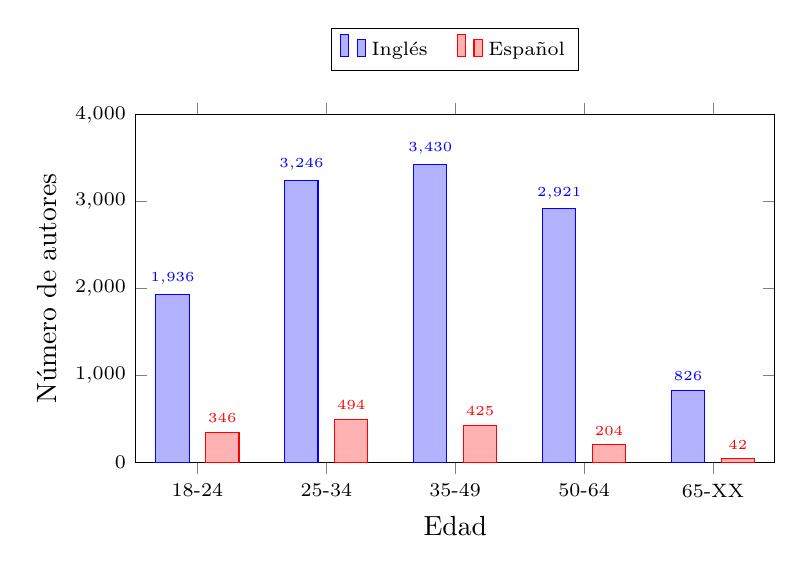
\begin{tikzpicture}
		\begin{axis}[
				width=0.8\textwidth,
				height=6cm,
				xmajorgrids=false,
				x tick label style={/pgf/number format/1000 sep=},
				x tick label style={font=\scriptsize},
				y tick label style={font=\scriptsize},
				ylabel=Número de autores,
				xlabel=Edad,
				ybar=6pt,
				bar width=12pt,
				enlarge x limits=0.12,
				nodes near coords,
				nodes near coords style={font=\tiny},
				symbolic x coords={18-24, 25-34, 35-49, 50-64, 65-XX},
				xtick=data,
				ymin=0,
				ymax=4000,
				legend style={at={(0.5,1.25)},font=\scriptsize, anchor=north,legend columns=-1, /tikz/every even column/.append style={column sep=0.3cm}},
			]
			\addplot table[x=Edad,y=Inglés] {
					Edad    Inglés
					18-24   1936
					25-34   3246
					35-49   3430
					50-64   2921
					65-XX   826
				};
			\addplot table[x=Edad,y=Español] {
					Edad    Español
					18-24   346
					25-34   494
					35-49   425
					50-64   204
					65-XX   42
				};
			\legend{Inglés, Español}
		\end{axis}
	\end{tikzpicture}
	\caption{Comparativa del número de autores por idioma en el \textit{corpus} del \textit{PAN Author Profiling 2014}}
	\label{fig:dataset_2014}
\end{figure}

\bigskip
\begin{table}[H]
	\centering
	\resizebox{0.7\textwidth}{!}{
		\rowcolors{2}{white}{udcgray!25}
		\begin{tabular}{|c|c|c|c|c|}
			\hhline{~|----|}
			\multicolumn{1}{c|}{\cellcolor{white}} & \multicolumn{2}{c|}{\cellcolor{udcpink!25}\textbf{Entrenamiento}} & \multicolumn{2}{c|}{\cellcolor{udcpink!25}\textbf{Test}}                                      \\ \hline
			\textbf{Edad}                          & \textbf{Inglés}                                                   & \textbf{Español}                                         & \textbf{Inglés} & \textbf{Español} \\ \hline
			18-24                                  & 1,936                                                             & 346                                                      & 850             & 158              \\ \hline
			25-34                                  & 3,246                                                             & 494                                                      & 1,380           & 218              \\ \hline
			35-49                                  & 3,430                                                             & 425                                                      & 1,470           & 210              \\ \hline
			50-64                                  & 2,921                                                             & 204                                                      & 1,226           & 92               \\ \hline
			65-XX                                  & 826                                                               & 42                                                       & 324             & 32               \\ \hline
			\textbf{Total}                         & \textbf{12,359}                                                   & \textbf{1,511}                                           & \textbf{5,250}  & \textbf{710}     \\ \hline
		\end{tabular}
	}
	\caption{Distribución del número de autores en cada rango de edad en el \textit{corpus} del \textit{PAN Author Profiling 2014}}
	\label{tab:dataset_2014}
\end{table}

\subsubsection{\textit{Resultados}}

Basándonos en los resultados de la competición, reflejados en la Tabla \ref{tab:algoritmos_2014}, podemos observar que los mejores datos de precisión
en cuanto a género fueron de alrededor de un 66\% para el inglés (precisión=0.6630) y de un 61\% para el español (precisión=0.6108), mientras que para la edad fueron de aproximadamente un 40\% para el inglés
(precisión=0.3950) y de un 50\% para el español (precisión=0.5010).

\bigskip
En cuanto a las aproximaciones algorítmicas llevadas a cabo por los equipos mejor clasificados en la competición, podemos destacar lo siguiente:

\begin{itemize}
	\item \textbf{Preprocesado}: En cuanto al preprocesado, tanto Maharjan et al. \cite{maharjan2014simple} como Weren et al. \cite{weren2014exploring} realizaron un limpiado de los documentos
	      (del inglés \textit{Extensible Markup Language}) para obtener texto plano, escapando caracteres inválidos en el caso del segundo equipo.
	\item \textbf{\textit{Features}}: En relación a las características extraídas de los documentos para la clasificación, Maharjan \cite{maharjan2014simple}, Weren et al. \cite{weren2014exploring} y Siang et al.,
	      consideraron diferentes rasgos estilométricos como la frecuencia de los signos de puntuación, el tamaño de las frases o la frecuencia de las palabras, entre otros. Con respecto
	      a los rasgos basados en el contenido, Siang et al. y Maharjan et al. \cite{maharjan2014simple}, modelizaron el lenguaje con \textit{bag-of-word} y n-gramas, respectivamente, mientras
	      que López-Monroy et al. \cite{lopez2014using} emplearon representaciones más complejas basadas en las relaciones entre palabras y documentos, explicadas a fondo
	      en su trabajo.
	\item \textbf{Clasificación}: En cuanto a los algoritmos de clasificación utilizados, todos los equipos que aparecen en la Tabla \ref{tab:algoritmos_2014} emplearon regresión logística. López-Monroy et al. \cite{lopez2014using}
	      hizo uso, más concretamente, de una librería de regresión logística y de SVMs lineales llamada LIBLINEAR (\textit{Large Linear Classification}) \cite{fan2008liblinear}.
\end{itemize}

\bigskip
\begin{table}[H]
	\centering
	\resizebox{0.9\textwidth}{!}{
		\rowcolors{2}{white}{udcgray!25}
		\setlength{\tabcolsep}{7pt}
		\begin{tabular}{|c|c|c|c|c|c|c|c|}
			\hhline{~|-------|}
			\multicolumn{1}{c|}{\cellcolor{white}}          & \multicolumn{7}{c|}{\cellcolor{udcpink!25}\textbf{Precisión}}                                                                                                                                                    \\
			\hhline{~|-------|}
			\multicolumn{1}{c|}{\cellcolor{white}}          & \multicolumn{3}{c|}{\textbf{Global}}                          & \multicolumn{2}{c|}{\textbf{Inglés}} & \multicolumn{2}{c|}{\textbf{Español}}                                                                     \\ \hline
			\textbf{Equipo participante}                    & \textbf{Conjunta}                                             & \textbf{Género}                      & \textbf{Edad}                         & \textbf{Género} & \textbf{Edad} & \textbf{Género} & \textbf{Edad} \\ \hline
			López-Monroy et al. 2014 \cite{lopez2014using}  & 0.2790                                                        & 0.6310                               & 0.4421                                & 0.6512          & 0.3950        & 0.6108          & 0.4892        \\ \hline
			Siang et al.                                    & 0.2758                                                        & 0.6344                               & 0.4348                                & 0.6630          & 0.3909        & 0.6057          & 0.4786        \\ \hline
			Maharjan et al., 2014 \cite{maharjan2014simple} & 0.2624                                                        & 0.5948                               & 0.4411                                & 0.6132          & 0.3811        & 0.5764          & 0.5010        \\ \hline
			Weren et al., 2014 \cite{weren2014exploring}    & 0.2266                                                        & 0.5866                               & 0.3863                                & 0.6066          & 0.3690        & 0.5666          & 0.4035        \\ \hline
		\end{tabular}
	}
	\caption{Cuatro mejores clasificados en la competición \textit{PAN Author Profiling 2014}}
	\label{tab:algoritmos_2014}
\end{table}

\subsection{\textit{PAN Author Profiling 2015}}
\label{sec:pan_2015}

En esta competición, a mayores de la clasificación por género y edad del autor, se añadió la predicción de rasgos de la personalidad. En concreto,
se buscaba predecir los cinco rasgos descritos en el modelo \textit{Big Five} (Goldberg, 1990) \cite{goldberg1990alternative}: extroversión (\textit{extroversion}),
estabilidad emocional / neuroticismo (\textit{stability / neuroticism}), apertura a la experiencia (\textit{openness to experience}), amabilidad (\textit{agreeableness}) y
responsabilidad (\textit{conscientiousness}). En cuanto a la edad, y a diferencia de la edición anterior de 2014, se eliminó la categoría de 65 años o más,
resultando en cuatro categorías: \textit{18-24}, \textit{25-34}, \textit{35-49} y \textit{50-XX}; donde esta última representa cualquier edad igual o superior
a los 50 años.

\subsubsection{\textit{Corpus}}
\label{sec:pan_2015_corpus}

\bigskip
En lo que respecta al \textit{corpus} proporcionado para la competición, los organizadores recopilaron \textit{tweets} de la red social Twitter
de 632 usuarios en cuatro idiomas diferentes: inglés, español, italiano y holandés. Dicho \textit{dataset} está etiquetado con el género y la edad
(solamente para inglés y español) de los autores, que ellos mismos reportaban en sus perfiles de Twitter. Para determinar los rasgos de la personalidad,
los autores completaron el test BFI-10 (Rammstedt et al., 2007) \cite{rammstedt2007measuring}, el cual proporcionaba valores para cada rasgo normalizados entre -0.5 y 0.5.
En este sentido, es importante destacar la gran reducción en cuanto al número de autores con los que cuenta el \textit{dataset} en comparación, por ejemplo,
con competicón celebrada en año anterior, la cual cuenta con cerca de 12,000. Esto puede generar problemas de sobreajuste (\textit{overfitting} en inglés) en los modelos
entrenados con esta colección, fenómeno que limita en gran medida la generalización y empeora notablemente los resultados en casso de uso reales.

\bigskip
Así, como se puede ver en la Figura \ref{fig:dataset_2015}, el \textit{dataset} vuelve a estar desbalanceado en cuanto a la edad, ya que existen
clases como la 50-XX la cual apenas cuenta con un un 7\% de representación. Sin embargo,
a excepción de la clase 18-24, existe un número similar de autores de habla española e inglesa, por lo que cabe esperar una generalización
semejante para ambos idiomas. En lo referente a la distribución de género, como se puede ver en la Tabla \ref{tab:dataset_2015}, está perfectamente balanceada,
contando con un 50\% de autores de cada género para todos los idiomas.

\bigskip
\begin{figure}[H]
	\centering
	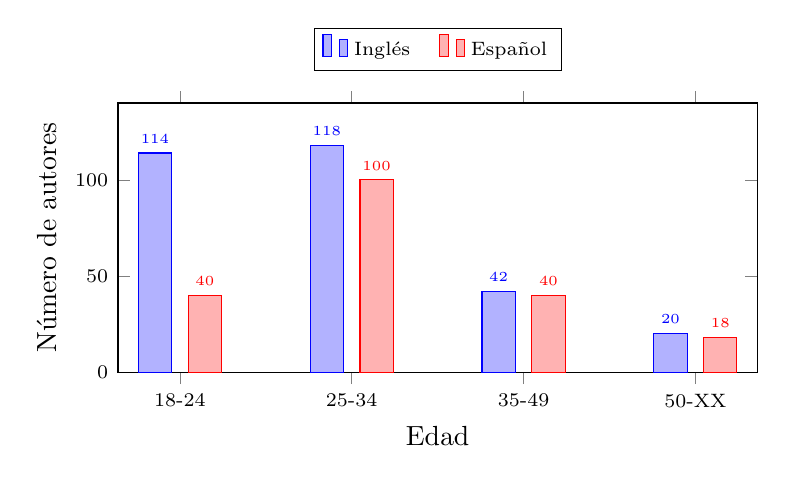
\begin{tikzpicture}
		\begin{axis}[
				width=0.8\textwidth,
				height=5cm,
				xmajorgrids=false,
				x tick label style={/pgf/number format/1000 sep=},
				x tick label style={font=\scriptsize},
				y tick label style={font=\scriptsize},
				ylabel=Número de autores,
				xlabel=Edad,
				ybar=6pt,
				bar width=12pt,
				enlarge x limits=0.12,
				nodes near coords,
				nodes near coords style={font=\tiny},
				symbolic x coords={18-24, 25-34, 35-49, 50-XX},
				xtick=data,
				ymin=0,
				ymax=140,
				legend style={at={(0.5,1.28)},font=\scriptsize, anchor=north,legend columns=-1, /tikz/every even column/.append style={column sep=0.3cm}},
			]
			\addplot table[x=Edad,y=Inglés] {
					Edad    Inglés
					18-24   114
					25-34   118
					35-49   42
					50-XX   20
				};
			\addplot table[x=Edad,y=Español] {
					Edad    Español
					18-24   40
					25-34   100
					35-49   40
					50-XX   18
				};
			\legend{Inglés, Español}
		\end{axis}
	\end{tikzpicture}
	\caption{Comparativa del número de autores por idioma en el \textit{corpus} del \textit{PAN Author Profiling 2015}}
	\label{fig:dataset_2015}
\end{figure}

\bigskip
\begin{table}[H]
	\centering
	\resizebox{0.9\textwidth}{!}{
		\rowcolors{2}{white}{udcgray!25}
		\setlength{\tabcolsep}{8pt}
		\begin{tabular}{|c|c|c|c|c|c|c|c|c|}
			\hhline{~|--------|}
			\multicolumn{1}{c|}{\cellcolor{white}} & \multicolumn{4}{c|}{\cellcolor{udcpink!25}\textbf{Entrenamiento}} & \multicolumn{4}{c|}{\cellcolor{udcpink!25}\textbf{Test}}                                                                                                                      \\ \hline
			\textbf{Característica}                & \textbf{Inglés}                                                   & \textbf{Español}                                         & \textbf{Italiano} & \textbf{Holandés} & \textbf{Inglés} & \textbf{Español} & \textbf{Italiano} & \textbf{Holandés} \\ \hline
			18-24                                  & 58                                                                & 22                                                       & -                 & -                 & 56              & 18               & -                 & -                 \\ \hline
			25-34                                  & 60                                                                & 56                                                       & -                 & -                 & 58              & 44               & -                 & -                 \\ \hline
			35-49                                  & 22                                                                & 22                                                       & -                 & -                 & 20              & 18               & -                 & -                 \\ \hline
			50-XX                                  & 12                                                                & 10                                                       & -                 & -                 & 8               & 8                & -                 & -                 \\ \hline
			\hline
			Masculino                              & 76                                                                & 55                                                       & 19                & 17                & 71              & 44               & 18                & 16                \\ \hline
			Femenino                               & 76                                                                & 55                                                       & 19                & 17                & 71              & 44               & 18                & 16                \\ \hline
			\hline
			Extrovertido                           & 0.16                                                              & 0.18                                                     & 0.17              & 0.24              & 0.17            & 0.16             & 0.15              & 0.24              \\ \hline
			Estabilidad                            & 0.14                                                              & 0.07                                                     & 0.20              & 0.21              & 0.13            & 0.09             & 0.20              & 0.22              \\ \hline
			Amabilidad                             & 0.12                                                              & 0.14                                                     & 0.22              & 0.13              & 0.14            & 0.14             & 0.19              & 0.15              \\ \hline
			Responsabilidad                        & 0.17                                                              & 0.24                                                     & 0.18              & 0.14              & 0.17            & 0.21             & 0.21              & 0.17              \\ \hline
			Apertura                               & 0.24                                                              & 0.18                                                     & 0.23              & 0.29              & 0.26            & 0.19             & 0.25              & 0.28              \\ \hline
		\end{tabular}
	}
	\caption{Distribución de los autores por característica y lenguaje en el \textit{corpus} del \textit{PAN Author Profiling 2015}}
	\label{tab:dataset_2015}
\end{table}

\subsubsection{\textit{Resultados}}

A la vista de los datos de precisión obtenidos por los primeros equipos clasificados, mostrados en la Tabla \ref{tab:algoritmos_2015},
podemos determinar que existe una gran mejora con respecto a los resultados de la competición anterior del año 2014, mejorando
la clasificación conjunta de edad y género en aproximadamente un 40\%.

\bigskip
Más en concreto, cabe destacar los grandes resultados que
ofrecen los algoritmos presentados con respecto al género en los dos idiomas principales del \textit{corpus}, llegando a alcanzar
precisiones del 96\% para el español en el caso de Alvarez-Carmona et al. \cite{alvarez2015inaoe} (precisión=0.9659). Con respecto a la edad,
se puede ver como se obtienen unos mejores resultados, de alrededor de un 5\%, en la clasificación en inglés que en español, algo que
hipotéticamente puede ser un reflejo de las pequeñas diferencias existentes entre el número de autores en cada uno de los idiomas en
el \textit{dataset} de entrenamiento. Sin embargo, estos tan buenos resultados, pueden ser también un reflejo del reducido número de
autores con los que cuenta el \textit{dataset}, de apenas 600 autores, lo que puede provocar un sobreajuste (\textit{overfitting} en inglés)
de los modelos.

\bigskip
Con respecto a la implementación de los algoritmos, podemos destacar lo siguiente:

\begin{itemize}
	\item \textbf{Preprocesado}: De forma similar a los algoritmos de años anteriores, la mayoría realizaron una limpieza del HTML incluído
	      en los \textit{tweets} y, tanto González-Gallardo et al. \cite{gonzalez2015tweets} como Grivas et al. \cite{grivas2015author}, utilizaron
	      las menciones, los \textit{hashtags} y los enlaces como características adicionales.
	\item \textbf{\textit{Features}}: En la mayor parte de los algoritmos presentados, se combinaba el uso de características
	      basadas en el estilo y en el contenido. Así, en cuanto a contenido, González-Gallardo et al. \cite{gonzalez2015tweets} hizo uso de n-gramas de caracteres
	      mientras que Grivas et al. \cite{grivas2015author} empleó TF-IDF con trigramas. Además, en el caso de Grivas et al. \cite{grivas2015author},
	      se analizaron otras características basadas en el estilo como la longitud de las palabras o el número de mayúsculas. En el caso de Alvarez-Carmona et al. \cite{alvarez2015inaoe},
	      se hizo uso del Análisis Semántico Latente, explicado en la Sección \ref{sec:analisis_semantico_latente}, junto a una técnica similar a la empleada por
	      López-Monroy et al. \cite{lopez2014using} en el año 2014.
	\item \textbf{Clasificación}: En lo referente a los métodos utilizados para realizar las predicciones, destaca el uso de la librería LIBLINEAR \cite{fan2008liblinear}
	      por parte de Alvarez-Carmona et al. \cite{alvarez2015inaoe} y González-Gallardo et al. \cite{gonzalez2015tweets}. En el caso de Grivas et al. \cite{grivas2015author}, se hizo
	      uso de SVMs para la clasificación del género y la edad mientras que se emplearon SVRs (Drucker et al., 1996) \cite{drucker1996support} para el reconocimiento de los rasgos personales.
\end{itemize}

\begin{table}[H]
	\centering
	\resizebox{\textwidth}{!}{
		\rowcolors{2}{white}{udcgray!25}
		\setlength{\tabcolsep}{6pt}
		\begin{tabular}{|c|c|c|c|c|c|c|c|c|c|}
			\hhline{~|---------|}
			\multicolumn{1}{c|}{\cellcolor{white}}                   & \multicolumn{9}{c|}{\cellcolor{udcpink!25}\textbf{Precisión}}                                                                                                                                                                                                                                        \\
			\hhline{~|---------|}
			\multicolumn{1}{c|}{\cellcolor{white}}                   & \multicolumn{3}{c|}{\textbf{Global}}                          & \multicolumn{2}{c|}{\textbf{Inglés}} & \multicolumn{2}{c|}{\textbf{Español}} & \multicolumn{1}{c|}{\textbf{Italiano}} & \multicolumn{1}{c|}{\textbf{Holandés}}                                                                       \\ \hline
			\textbf{Equipo participante}                             & \textbf{Conjunta}                                             & \textbf{Género}                      & \textbf{Edad}                         & \textbf{Género}                        & \textbf{Edad}                          & \textbf{Género} & \textbf{Edad} & \textbf{Género} & \textbf{Género} \\ \hline
			Alvarez-Carmona et al. 2015 \cite{alvarez2015inaoe}      & 0.7116                                                        & 0.8712                               & 0.8168                                & 0.8592                                 & 0.8380                                 & 0.9659          & 0.7955        & 0.7222          & 0.9375          \\ \hline
			González-Gallardo et al., 2015 \cite{gonzalez2015tweets} & 0.6693                                                        & 0.8871                               & 0.7545                                & 0.8521                                 & 0.7817                                 & 0.8977          & 0.7273        & 0.8611          & 0.9375          \\ \hline
			Grivas et al., 2015 \cite{grivas2015author}              & 0.6487                                                        & 0.9011                               & 0.7199                                & 0.8592                                 & 0.7465                                 & 0.9432          & 0.6932        & 0.8333          & 0.9688          \\ \hline
			Kocher et al., 2015 \cite{kocher2015unine}               & 0.5655                                                        & 0.7800                               & 0.7250                                & 0.7113                                 & 0.7113                                 & 0.8182          & 0.7386        & 0.7778          & 0.8125          \\ \hline
		\end{tabular}
	}
	\caption{Cuatro mejores clasificados en la competición \textit{PAN Author Profiling 2015}}
	\label{tab:algoritmos_2015}
\end{table}

\subsection{\textit{PAN Celebrity Profiling 2019}}

En esta última competición analizada, la primera de ellas celebrada específicamente para el perfilado de celebridades, la tarea consistía en predecir
cuatro características demográficas a partir de sus publicaciones en Twitter:

\begin{itemize}
	\item \textbf{Género}: Masculino, femenino o no binario.
	\item \textbf{Año de nacimiento}: A la hora de calcular la precisión del algoritmo,
	      se contempló una ventana de error adaptativa, entre los 2 y los 9 años, en función de la edad real de la celebridad.
	\item \textbf{Ocupación o motivo de fama}: Deportista (\textit{sports}), actor (\textit{performer}), político (\textit{politics}), creador de contenido (\textit{creator}),
	      director (\textit{manager}), científico (\textit{science}), profesional (\textit{professional}) o religioso (\textit{religious}).
	\item \textbf{Fama}: Revelación (\textit{rising}), estrella (\textit{star}) o superestrella (\textit{superstar}), determinado en función del número de seguidores en Twitter.
\end{itemize}

\subsubsection{\textit{Corpus}}

Como se mencionó anteriormente, el \textit{corpus} empleado está compuesto por publicaciones en inglés de celebridades en la red social Twitter.
En este caso, un usuario era considerado una celebridad si tenía un perfil verificado en Twitter y superaba cierto umbral
de notoriedad en Wikidata \cite{wikidata}. El \textit{corpus},
que contenía un total de 48.335 celebridades con aproximadamente 2.180 \textit{tweets} cada una, fue obtenido
a partir del \textit{Webis Celebrity Profiling Corpus} (Wiegmann et al., 2019) \cite{wiegmann2019celebrity}, en el cual se relacionaban los perfiles
de Twitter de cada celebridad con sus entradas en Wikidata. De esta forma, se obtuvieron los \textit{tweets} de la red social
y se simplificaron las características demográficas que ofrecía Wikidata, excluyendo las celebridades nacidas antes de 1940 y que no tuvieran
el inglés como lengua de uso principal. Finalmente, para generar un conjunto de entrenamiento y otro de validación, se optó por una división
70-30, obteniendo 33.836 y 14.499 celebridades para cada uno, respectivamente.

\bigskip
Con todo, las distribuciones de las celebridades en las distintas características demográficas se muestran en las Figuras \ref{fig:distribuciones_genero_fama_2019},
\ref{fig:distribucion_ocupacion_2019} y \ref{fig:distribucion_edad_2019}. Como se puede observar, existe un gran desbalanceo
en el género, fama y ocupación, propiciando un posible sesgo hacia las clases mayoritarias (masculino, estrella y deportista) en las predicciones de los algoritmos.
En lo que respecta al año de nacimiento,
la mayor parte se concentran alrededor de los años 80 y 90, acumulando un 50\% de las celebridades.
Además, como se puede ver en dicho gráfico, existe una anomalía
para el año 2000, la cual se debe a un error de los datos proporcionados por Wikidata, según apunta la organización de la competición.

\bigskip
\begin{figure}[H]
	\centering
	\begin{subfigure}{0.5\textwidth}
		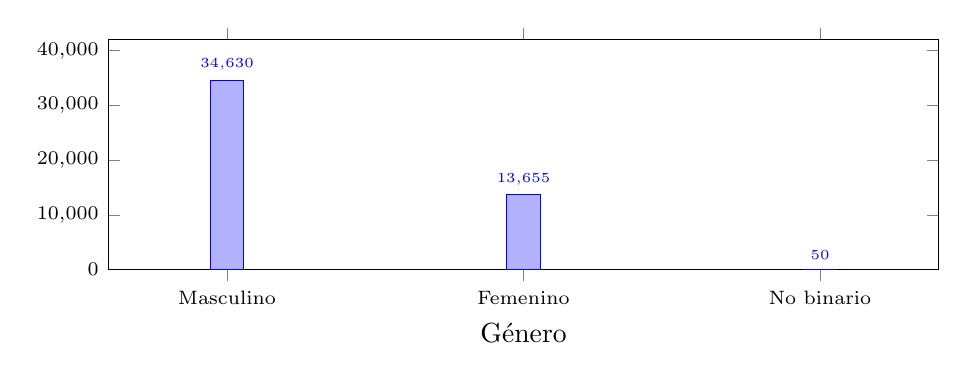
\begin{tikzpicture}
			\begin{axis}[
					width=\linewidth,
					height=4.5cm,
					xmajorgrids=false,
					x tick label style={font=\scriptsize},
					y tick label style={font=\scriptsize},
					ybar=6pt,
					bar width=12pt,
					enlarge x limits=0.2,
					ymin=0,
					ymax=42000,
					nodes near coords,
					nodes near coords style={font=\tiny},
					xtick=data,
					xticklabels={Masculino, Femenino, {No binario}},
					xlabel={Género},
					scaled y ticks=false
				]
				\addplot coordinates {(1,34630) (2,13655) (3,50)};
			\end{axis}
		\end{tikzpicture}
		\label{fig:distribucion_genero_2019}
	\end{subfigure}%
	\hfill
	\begin{subfigure}{0.5\textwidth}
		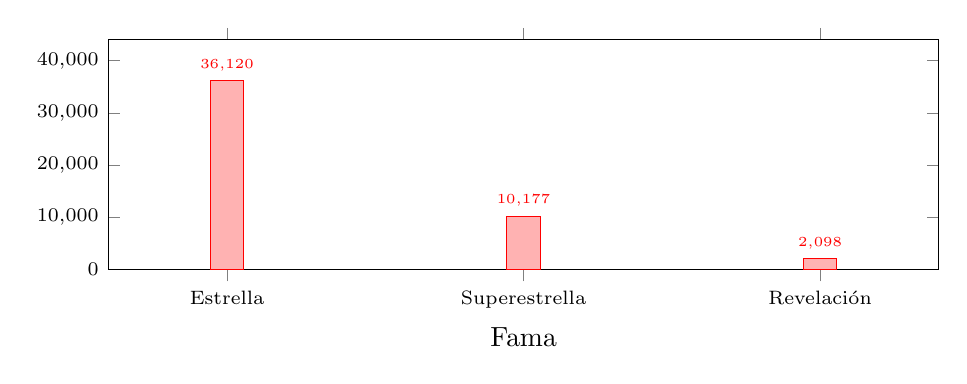
\begin{tikzpicture}
			\begin{axis}[
					width=\linewidth,
					height=4.5cm,
					xmajorgrids=false,
					x tick label style={font=\scriptsize},
					y tick label style={font=\scriptsize},
					ybar=6pt,
					bar width=12pt,
					enlarge x limits=0.2,
					ymin=0,
					ymax=44000,
					nodes near coords,
					nodes near coords style={font=\tiny},
					xtick=data,
					xticklabels={Estrella, Superestrella, Revelación},
					xlabel={Fama},
					scaled y ticks=false
				]
				\addplot[color=red, fill=red!30] coordinates {(1,36120) (2,10177) (3,2098)};
			\end{axis}
		\end{tikzpicture}
		\label{fig:distribucion_fama_2019}
	\end{subfigure}
	\caption{Distribuciones de género y fama en el \textit{corpus} de la competición \textit{PAN Celebrity Profiling 2019}.}
	\label{fig:distribuciones_genero_fama_2019}
\end{figure}

\begin{figure}[H]
	\centering
	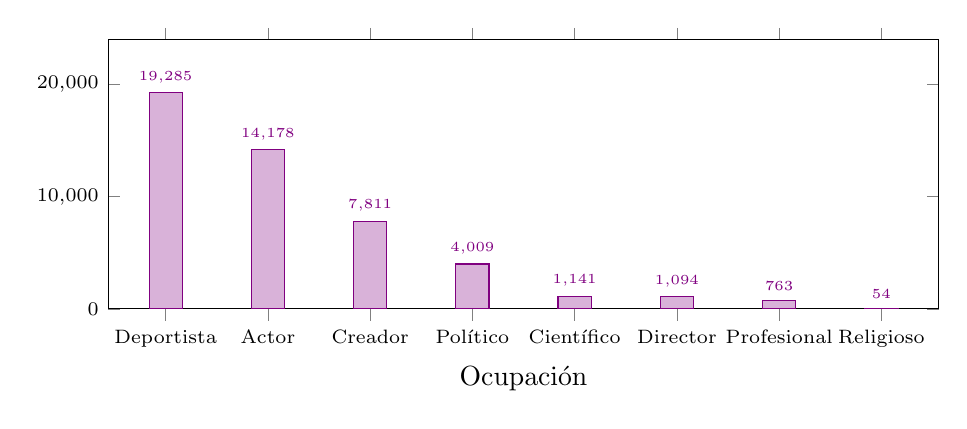
\begin{tikzpicture}
		\begin{axis}[
				width=\linewidth,
				height=5cm,
				xmajorgrids=false,
				x tick label style={font=\scriptsize},
				y tick label style={font=\scriptsize},
				ybar=6pt,
				bar width=12pt,
				enlarge x limits=0.08,
				ymin=0,
				ymax=24000,
				nodes near coords,
				nodes near coords style={font=\tiny},
				xtick=data,
				xticklabels={Deportista, Actor, Creador, Político, Científico, Director, Profesional, Religioso},
				xlabel={Ocupación},
				scaled y ticks=false
			]
			\addplot[color=violet, fill=violet!30] coordinates {(1,19285) (2,14178) (3,7811) (4,4009) (5,1141) (6,1094) (7,763) (8,54)};
		\end{axis}
	\end{tikzpicture}
	\caption{Distribución de ocupaciones en el \textit{corpus} de la competición \textit{PAN Celebrity Profiling 2019}.}
	\label{fig:distribucion_ocupacion_2019}
\end{figure}

\begin{figure}[H]
	\centering
	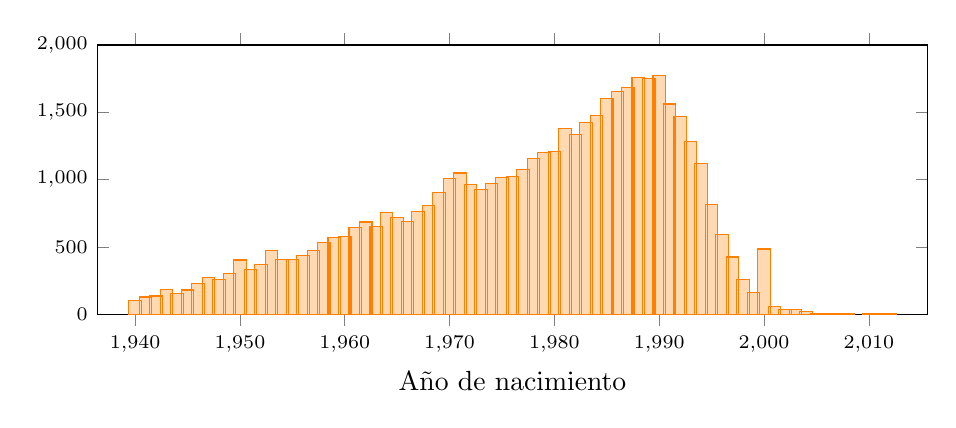
\begin{tikzpicture}
		\begin{axis}[
				width=\textwidth,
				height=5cm,
				xmajorgrids=false,
				x tick label style={font=\scriptsize},
				y tick label style={font=\scriptsize},
				ybar=1pt,
				bar width=4.5pt,
				enlarge x limits=0.05,
				ymin=0,
				ymax=2000,
				xlabel={Año de nacimiento},
				scaled y ticks=false
			]
			\addplot[color=orange, fill=orange!30] coordinates {(1940,105) (1941,128) (1942,135) (1943,182)
					(1944,154) (1945,180) (1946,225) (1947,274) (1948,260) (1949,304) (1950,403) (1951,333)
					(1952,368) (1953,470) (1954,405) (1955,407) (1956,436) (1957,472) (1958,532) (1959,568)
					(1960,579) (1961,642) (1962,685) (1963,649) (1964,756) (1965,716) (1966,689) (1967,760)
					(1968,805) (1969,907) (1970,1010) (1971,1049) (1972,963) (1973,927) (1974,973) (1975,1014)
					(1976,1021) (1977,1075) (1978,1159) (1979,1202) (1980,1206) (1981,1377) (1982,1336) (1983,1424)
					(1984,1475) (1985,1604) (1986,1654) (1987,1682) (1988,1759) (1989,1748) (1990,1771) (1991,1562)
					(1992,1467) (1993,1286) (1994,1118) (1995,816) (1996,595) (1997,425) (1998,258) (1999,160)
					(2000,484) (2001,57) (2002,33) (2003,34) (2004,20) (2005,6) (2006,2) (2007,5) (2008,1) (2010,2) (2011,1) (2012,1)};
		\end{axis}
	\end{tikzpicture}
	\caption{Distribución del año de nacimiento en el \textit{corpus} de la competición \textit{PAN Celebrity Profiling 2019}.}
	\label{fig:distribucion_edad_2019}
\end{figure}


\subsubsection{\textit{Resultados}}

Como se aprecia en la Tabla \ref{tab:algoritmos_2019}, la precisión conjunta en edad y género obtenida por los algoritmos mejor
clasificados es de aproximadamente un 20\% inferior a la alcanzada en la competición del año 2015. Esto es debido a que,
como se comentó anteriormente, la clasificación de edad no se realizó en base a rangos en esta edición, sino que se
buscó una predicción exacta de la edad del autor, junto a una grado de tolerancia adaptativo, provocando así precisiones mucho
más bajas para este atributo. {\color{red}En lo que respecta a la clasificación del género, vemos como los dos
mejores participantes obtienen resultados de aproximadamente un 90\%, superior a los obtenidos en la edición de 2015.
Por último, en cuanto a la clasificación de ocupación, destacar el gran resultado que ofrece el algoritmo de Radivchev et al. \cite{radivchev2019celebrity},
obteniendo una precisión del 75\% para una característica con ocho clases diferentes (precisión=0.757)}.

\bigskip
Centrándonos en las implementaciones realizadas en esta competición, podemos destacar lo siguiente:

\begin{itemize}
	\item \textbf{Preprocesado}: Para el preprocesado, Martinc et al. \cite{martinc2019hot}, Radivchev et al. \cite{radivchev2019celebrity}
	      y Moreno-Sandoval et al. \cite{moreno2019celebrity}, optaron por sustituír los enlaces,
	      las menciones y los \textit{hashtags} por etiquetas especiales. Por otro lado, Martinc et al. \cite{martinc2019hot} se decantó por eliminar los signos de puntuación
	      y las \textit{stopwords}, es decir, las palabras poco significativas, para mejorar el modelado de los documentos con TF-IDF puro basado en unigramas de palabras.
	\item \textbf{\textit{Features}}: La mayor parte de los algoritmos presentados emplearon técnicas basadas en TF-IDF y n-gramas.
	      Más concretamente, Radivchev et al. \cite{radivchev2019celebrity} utilizó como características los vectores obtenidos mediante TF-IDF sobre los 10.000 bigramas más frecuentes;
	      Martinc et al. \cite{martinc2019hot} obtuvo los vectores mediante el TF-IDF de unigramas de palabras y tetragramas de caracteres; Moreno-Sandoval et al. \cite{moreno2019celebrity}, en cambio, además de
	      de emplear n-gramas como características, calculó el número medio de emojis, \textit{hashtags}, meciones, enlaces, \textit{retweets}, palabras y longitud de las
	      palabras por \textit{tweet}.
	\item \textbf{Clasificación}: Al igual que en las pasadas ediciones, los métodos de clasificación más frecuentes fueron las
	      SVMs y la regresión logística. Radivchev et al. \cite{radivchev2019celebrity} utilizó SVMs para la predicción de la fama y la ocupación, mientras que para la edad y género
	      hizo uso de la regresión logística; Moreno-Sandoval et al. \cite{moreno2019celebrity}, en cambio, empleó la regresión logística para la clasificación de todos los atributos
	      excepto para la ocupación, que obtuvo mejores resultados haciendo uso de un clasificador multinomial Bayesiano Ingenuo (\textit{Multinomial Naive Bayes} o MNB en inglés).
	      Por último, Martinc et al. \cite{martinc2019hot} empleó regresión logística para la clasificación de las cuatro características demográficas.
\end{itemize}

\begin{table}[H]
	\centering
	\resizebox{0.9\textwidth}{!}{
		\rowcolors{2}{white}{udcgray!25}
		\setlength{\tabcolsep}{6pt}
		\begin{tabular}{|c|c|c|c|c|c|}
			\hhline{~|-----|}
			\multicolumn{1}{c|}{\cellcolor{white}}                  & \multicolumn{5}{c|}{\cellcolor{udcpink!25}\textbf{Precisión}}                                                                        \\ \hline
			\textbf{Equipo participante}                            & \textbf{Conjunta} (Género y Edad)                             & \textbf{Género} & \textbf{Edad} & \textbf{Ocupación} & \textbf{Fama} \\ \hline
			Radivchev et al. 2019 \cite{radivchev2019celebrity}     & 0.477                                                         & 0.928           & 0.514         & 0.757              & 0.777         \\ \hline
			Martinc et al., 2019 \cite{martinc2019hot}              & 0.410                                                         & 0.906           & 0.453         & 0.732              & 0.755         \\ \hline
			Fernquist et al., 2019                                  & 0.362                                                         & 0.774           & 0.468         & 0.642              & 0.773         \\ \hline
			Moreno-Sandoval et al., 2019 \cite{moreno2019celebrity} & 0.320                                                         & 0.862           & 0.371         & 0.703              & 0.545         \\ \hline
		\end{tabular}
	}
	\caption{Cuatro mejores clasificados en la competición \textit{PAN Celebrity Profiling 2019}}
	\label{tab:algoritmos_2019}
\end{table}

\subsection{Conclusiones}

Tras el análisis de estas tres competiciones, en lo que concierne al objetivo de este trabajo,
podemos concluir que la clasificación tanto del de género como de la edad son tareas
que ofrecen resultados sorprendentes, llegando a superar precisiones de hasta un 90\% en el caso del género y un 80\% en el caso de la edad,
convirtiéndose así en herramientas de gran fiabilidad para el perfilado automático de autores.

\bigskip
En lo que respecta a los algoritmos, no apreciamos grandes diferencias entre ediciones, ya que el preprocesado sigue involucrando
el limpiado del texto, la eliminación de palabras poco significativas o la sustitución de ciertos elementos por \textit{tokens} especiales;
las características continúan estando basadas en medidas estadísticas como el TF-IDF y los n-gramas, junto
a otras que se apoyan en rasgos estilísticos como la media de palabras o el número de signos de puntuación; y los métodos de clasificación más utilizados
siguen estando fundamentados en técnicas de aprendizaje supervisado clásicas como los SVMs y la regresión logística.

\bigskip
En este sentido, autores de las competiciones más recientes como Martinc et al., 2019 \cite{martinc2019hot} o Radivchev et al., 2019 \cite{radivchev2019celebrity}, destacan
la gran efectividad que tienen estos métodos clásicos
con respecto a técnicas más modernas como las basadas en Aprendizaje Profundo (\textit{Deep Learning} en inglés). Martinc et al., 2019 \cite{martinc2019hot}, por ejemplo,
apunta que, haciendo uso de BERT, una red neuronal basada en Transformers propuesta por Devlin et al., 2018 \cite{devlin2018bert},
los resultados obtenidos fueron significativamente peores en comparación con la regresión logistica, de alrededor de un 10\% en F1. En el caso
de Radivchev et al., 2019 \cite{radivchev2019celebrity}, se reportaron resultados similares, en este caso haciendo uso de DPCNN (\textit{Deep Pyramid Convolutional Neural Network} en inglés),
propuesta por Johnson et al., 2017 \cite{johnson2017deep} para el procesado de textos.

\section{Algoritmos seleccionados}
\label{sec:algoritmos_seleccionados}

Con todo, para seleccionar los algoritmos que formarán parte de la aplicación que se expondrá en los siguientes capítulos, se ha optado
por buscar aquellos que contasen con una implementación pública y que, además, ofreciesen un buen rendimiento en las competiciones.
Por ello, dado que los algoritmos de la edición de 2014 no obtenían restulados comparables a las otras dos competiciones,
no se ha tenido en cuenta ninguno de ellos. Así, de los cuatro algoritmos mejor clasificados del \textit{PAN Author Profiling 2015} y
del \textit{PAN Celebrity Profiling 2019} se ha seleccionado uno de cada competición, concretamente las implementaciones propuestas por
Grivas et al. \cite{grivas2015author} (disponible en \url{https://github.com/pan-webis-de/grivas15})
y Martinc et al. \cite{martinc2019hot} (disponible en \url{https://github.com/EMBEDDIA/PAN2019}).

\subsection{Algoritmo de Grivas et al. \cite{grivas2015author}}

Este algoritmo sigue una aproximación particular basada en la creación de dos grupos de características, unas basadas en el contenido (estructurales) y otras basadas en el estilo (estilométricas).
Como se puede ver en la Figura \ref{fig:features_grivas}, las características estructurales se corresponden con el número de \textit{hashtags}, enlaces y menciones que aparecen en los \textit{tweets},
mientras que las características estilométricas se corresponden con algunas más comunes como el TF-IDF de n-gramas o el número de mayúsculas junto con otras menos
utilizadas como la bolsa de emoticonos (\textit{bag-of-smileys} en inglés), una técnica similar a la \textit{bag-of-words} explicada en la Sección \ref{sec:bag_of_words} o los grafos de n-gramas, propuestos
por Giannakopoulos et al., 2008 \cite{giannakopoulos2008summarization}.

\bigskip
\begin{figure}[H]
	\centering
	\resizebox{0.8\textwidth}{!}{
		\begin{forest}
			for tree={
			draw,
			element,
			parent anchor=east,
			child anchor=west,
			grow=east,
			align=center,
			base=bottom,
			edge={->},
			l sep+=10mm,
			font=\sffamily,
			text width=4cm
			},
			[Características, fill=orange!20
			[Estructurales, for tree={fill=red!20}
				[Número de \textit{hashtags}]
				[Número de enlaces]
				[Número de menciones]
			]
			[Estilométricas, for tree={fill=blue!20}
				[TF-IDF de n-gramas]
				[\textit{Bag-of-smileys}]
				[Grafos de n-gramas]
				[Longitud de palabras]
				[Número de mayúsculas]
			]
			]
		\end{forest}
	}
	\caption{Características extraídas en el algoritmo de Grivas et al. \cite{grivas2015author}, }
	\label{fig:features_grivas}
\end{figure}

\bigskip
A mayores, para cada uno de los grupos de \textit{features}, se aplicaron preprocesados diferentes debido a la naturaleza de las propias características. De esta forma, para la extracción del grupo de \textit{features}
estructurales, no se realizó nigún tipo de preprocesado. Sin embargo, para reducir el ruido en el grupo de \textit{features} estilométricas, se eliminó cualquier tipo de HTML presente en los \textit{tweets}, ignorando así
elementos como las menciones o los enlaces.

\bigskip
Por otro lado, como se muestra en la Tabla \ref{tab:features_per_task_grivas}, solo algunas de las características extraídas anteriormente son utilizadas en cada una de las subtareas, basándose
para ello en una serie de heurísticas y de pruebas realizadas con el \textit{dataset} de entrenamiento.

\bigskip
\begin{table}[H]
	\centering
	\resizebox{0.9\textwidth}{!}{
		\rowcolors{2}{white}{udcgray!25}
		\begin{tabular}{|c|p{4cm}|p{4cm}|}
			\hhline{~|--|}
			\multicolumn{1}{c|}{\cellcolor{white}} & \multicolumn{2}{c|}{\cellcolor{udcpink!25}\textbf{Grupo de características}}                                                                                          \\ \hline
			\textbf{Subtarea}                      & \textbf{Estructurales}                                                              & \textbf{Estilométricas}                                                         \\ \hline
			Género                                 & -                                                                                   & TF-IDF de trigramas                                                             \\ \hline
			Edad                                   & Número de menciones \newline Número de \textit{hashtags} \newline Número de enlaces & TF-IDF de trigramas \newline Longitud de palabras                               \\ \hline
			Rasgos personales                      & Número de menciones \newline Número de \textit{hashtags} \newline Número de enlaces & TF-IDF de trigramas	\newline Longitud de palabras \newline Número de mayúsculas \\ \hline
		\end{tabular}
	}
	\caption{Características extraídas en el algoritmo de Grivas et al. \cite{grivas2015author}}
	\label{tab:features_per_task_grivas}
\end{table}

\bigskip
Finalmente, en lo que concierne a las técnicas de clasificación, se utilizaron SVMs con un kernel RBF (\textit{Radial Basis Function} en inglés) y con un kernel lineal
para las subtareas de predicción de la edad y el género, respectivamente. En el caso de la predicción de los rasgos personales, se empleó un SVR (\textit{Support Vector Regression} en inglés)
con un kernel lineal. Destacar que, para la ejecución de ambos algoritmos de aprendizaje automático, se hizo uso de las librerías ofrecidas por scikit-learn \cite{scikitlearn}.

\subsection{Algoritmo de Martinc et al. \cite{martinc2019hot}}

En lo que respecta a este segundo algoritmo seleccionado, lo primero que se realiza es un concatenado de los primeros 100 \textit{tweets} de cada usuario para la creación de cada documento
que formará la colección. La razón de este límite se justifica en la reducción considerable de la complejidad temporal y espacial, manteniendo a su vez una muestra representativa que garantiza
una buena clasificación.

\bigskip
Una vez realizado este paso, se continúa con el preprocesado de los documentos, el cual se divide en tres niveles incrementales, como se aprecia en la Figura \ref{fig:preprocesado_martinc}.

\bigskip
\begin{figure}[H]
	\centering
	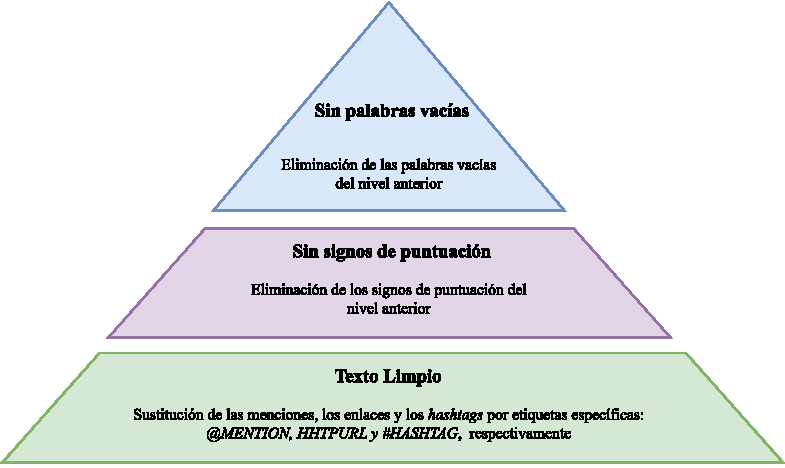
\includegraphics[width=0.8\textwidth]{diagramas/pyramid-martinc.pdf}
	\caption{Niveles del preprocesado en el algoritmo de Martinc et al. \cite{martinc2019hot}}
	\label{fig:preprocesado_martinc}
\end{figure}

Posteriormente, en la fase de extracción de características, se obtuvieron diferentes vectores de n-gramas basados en TF-IDF, calculados cada uno sobre un nivel diferente de preprocesado:

\bigskip
\begin{itemize}
	\item \textbf{Unigramas de palabras}: Calculado sobre el documento del Nivel 3 (sin palabras vacías) transformado a minúsculas.
	\item \textbf{Tetragramas de caracteres}: Calculado sobre el documento del Nivel 1 (texto limpio) transformado a minúsculas.
	\item \textbf{Tetragramas de caracteres sufijos}: Calculado sobre el documento del Nivel 1 (texto limpio) transformado a minúsculas. Aclarar que para esta representación
	      se cosideran las cuatro últimas letras de cada palabra con una longitud suficiente, es decir, sufijos de cuatro caracteres.
\end{itemize}

Finalmente, se hicieron pruebas con varios clasificadores, entre ellos SVMs con diferentes \textit{kernels}, \textit{random forest} o \textit{gradient boosting}, pero el que mejores resultados
obtuvo fue el de regresión logística, siendo empleado en todas las subtareas de clasificación de la competición. Para hallar dicha solución y obtener los hiparámetros óptimos para cada
clasificador, se aplicó una búsqueda en rejilla (\textit{grid search} en inglés), en la que se evaluaron todas las posibles combinaciones de parámetros.
Destacar también el uso de la clase \textit{FeatureUnion} de scikit-learn \cite{scikitlearn}, la cual permite la concatenación de diferentes características en un mismo vector asignándoles
un diferente peso a cada una de ellas, obteniendo para este caso un peso de 0.8 sobre 1.0 para los unigramas de palabras y los tetragramas de caracteres, mientras que tan solo un 0.4 para los tetragramas de caracteres sufijos,
lo que implica una menor relevancia.

\subsection{Pruebas}

Una vez seleccionados los algoritmos y explicado su funcionamiento, es necesario llevar a cabo una serie de pruebas que nos permitan determinar
si obtienen los mismos resultados en la clasificación que los reportados en sus respectivos trabajos.
Para ello, se hará uso de los \textit{datasets} de entrenamiento y test originales que proporcionaba públicamente cada competición disponibles
en \url{https://zenodo.org/record/3745945} y \url{https://zenodo.org/record/3885373} para las ediciones de 2015 y 2019, respectivamente.

\bigskip
En cuanto al algoritmo de Grivas et al. \cite{grivas2015author}, como se observa en la Tabla \ref{tab:pruebas_grivas}, existen pequeñas variaciones en
cuanto a la precisión, cerca de un 4.7\%, lo que se puede deber a cambios en el propio \textit{dataset} de entrenamiento o test ofrecidos. A mayores,
se muestra una columna con el macro F1 obtenido. Esta métrica, basada en el F1 tradicional, se calcula como la media de los F1 de cada clase,
reflejando los problemas subyacentes en casos de conjuntos de entrenamiento desbalanceados.
Así, vemos como los resultados obtenidos para el género son buenos, mientras que para la edad son bastante peores. Esto puede deberse al gran
desbalanceo de clases de la edad, junto a las pequeñas diferencias que pueden existir entre rangos contiguos y que provocan errores en la clasificación.

\bigskip
\begin{table}[H]
	\centering
	\resizebox{0.7\textwidth}{!}{
		\rowcolors{2}{white}{udcgray!25}
		\begin{tabular}{|c|c|c|c|}
			\hhline{~|---|}
			\multicolumn{1}{c|}{\cellcolor{white}} & \multicolumn{2}{c|}{\cellcolor{udcpink!25}\textbf{Precisión}} & \multicolumn{1}{c|}{\cellcolor{udcpink!25}\textbf{Macro F1}}                     \\ \hline
			\textbf{Característica}                & \textbf{Reportada}                                            & \textbf{Obtenida}                                            & \textbf{Obtenida} \\ \hline
			Género                                 & 0.8592                                                        & 0.8310                                                       & 0.8304            \\ \hline
			Edad                                   & 0.7465                                                        & 0.7887                                                       & 0.5631            \\ \hline
		\end{tabular}
	}
	\caption{Resultados de las pruebas realizadas con el algoritmo de Grivas et al. \cite{grivas2015author}}
	\label{tab:pruebas_grivas}
\end{table}

\bigskip
A mayores, ya que los \textit{datasets} de la edición de 2014 y de 2015 tienen una estructura similar, permitió utilizar la colección
del \textit{PAN Author Profiling 2014}, disponible en \url{https://zenodo.org/record/3716008}, para llevar a cabo experimentos y comparar los resultados que ofrece el algoritmo
de Grivas et al. \cite{grivas2015author} con cada uno. Con todo, fue necesario realizar las siguientes modificaciones para que, tanto el algoritmo
como la colección, fuesen completamente compatibles:

\begin{itemize}
	\item \textbf{Transformación de etiquetas}: Para que el conjunto de clases presentes en cada subtarea fuese el mismo que el presentado en la edición de 2015, se modificaron
	      las etiquetas del fichero de \textit{truth}. De este modo, en el caso de la edad, se agruparon los rangos 50-64 y 65-XX en uno solo (50-XX), mientras que en el género se sustituyeron
	      las etiquetas \textit{MALE} y \textit{FEMALE} por sus iniciales.
	\item \textbf{Modificación de código}: En cuanto al código fuente, fue necesario ignorar todo lo referente a la subtarea de la predicción de los rasgos de la personalidad
	      expuesta en la competición de 2015, ya que el \textit{dataset} de 2014 no contaba con dichas características.
\end{itemize}

\bigskip
De esta forma, haciendo uso del \textit{dataset} de 2014 para entrenar el algoritmo de Grivas et al. \cite{grivas2015author}, se obtuvieron los resultados
mostrados en la Tabla \ref{tab:pruebas_grivas_PAN14}. Destacar que, debido a que la colección proporcionada en 2014 no contaba con un conjunto específico de test, se realizó la validación
con el conjunto de test de la competición de 2015, obteniendo así resultados directamente comparables con los reportados en la Tabla \ref{tab:pruebas_grivas}.
En este sentido, vemos como la precisión y el F1 de ambas características se reduce drásticamente a causa, hipotéticamente, de dos factores. El primero de ellos
tiene que ver con heterogeneidad de los textos en el conjunto de entrenamiento, ya que se unificaron las publicaciones de los blogs, las \textit{reviews} de hoteles y
los \textit{posts} de otras redes sociales, provocando, por un lado, una dificultad añadida en el proceso de extracción de características y, por otro lado,
un gran contraste con los \textit{tweets} utilizados para la validación. El segundo factor tiene que ver con la gran diferencia en el tamaño de los \textit{datasets},
dado que la edición de 2014 contaba con 12,053 autores frente a 142 de la de 2015.

\bigskip
\begin{table}[H]
	\centering
	\resizebox{0.6\textwidth}{!}{
		\rowcolors{2}{white}{udcgray!25}
		\begin{tabular}{|c|c|c|}
			\hhline{~|--|}
			\multicolumn{1}{c|}{\cellcolor{white}} & \multicolumn{2}{c|}{\cellcolor{udcpink!25}\textbf{Colección del PAN 2014}}                     \\ \hline
			\textbf{Característica}                & \textbf{Precisión}                                                         & \textbf{Macro F1} \\ \hline
			Género                                 & 0.6408                                                                     & 0.6328            \\ \hline
			Edad                                   & 0.5282                                                                     & 0.3587            \\ \hline
		\end{tabular}
	}
	\caption{Resultados de las pruebas realizadas con el \textit{dataset} de 2014 para el algoritmo de Grivas et al. \cite{grivas2015author}}
	\label{tab:pruebas_grivas_PAN14}
\end{table}

\bigskip
En la misma línea, el algoritmo de Martinc et al. \cite{martinc2019hot} también obtiene resultados muy similares como se muestra en la Tabla \ref{tab:pruebas_martinc},
con una variación del 1.4\% en la precisión y del 7.4\%, algo más elevadas, en el macro F1. Destacar que, para esta última métrica, al algoritmo obtiene
resultados bastante pobres en comparación con la precisión, lo que demuestra un posible sesgo hacia las clases mayoritarias en el conjunto de entrenamiento.

\bigskip
\begin{table}[H]
	\centering
	\resizebox{0.7\textwidth}{!}{
		\rowcolors{2}{white}{udcgray!25}
		\setlength{\tabcolsep}{8pt}
		\begin{tabular}{|c|c|c|c|c|}
			\hhline{~|----|}
			\multicolumn{1}{c|}{\cellcolor{white}} & \multicolumn{2}{c|}{\cellcolor{udcpink!25}\textbf{Precisión}} & \multicolumn{2}{c|}{\cellcolor{udcpink!25}\textbf{Macro F1}}                                          \\ \hline
			\textbf{Característica}                & \textbf{Reportada}                                            & \textbf{Obtenida}                                            & \textbf{Reportada} & \textbf{Obtenida} \\ \hline
			Género                                 & 0.906                                                         & 0.904                                                        & 0.587              & 0.584             \\ \hline
			Edad                                   & 0.453                                                         & 0.433                                                        & 0.354              & 0.308             \\ \hline
			Fama                                   & 0.755                                                         & 0.755                                                        & 0.512              & 0.480             \\ \hline
			Ocupación                              & 0.743                                                         & 0.731                                                        & 0.468              & 0.427             \\ \hline
		\end{tabular}
	}
	\caption{Resultados de las pruebas realizadas con el algoritmo de Martinc et al. \cite{martinc2019hot}}
	\label{tab:pruebas_martinc}
\end{table}

Sin embargo, ya que la utilidad real de la predicción exacta del año de nacimiento para el perfilado de autores es limitada,
se buscó mejorar la precisión del algoritmo mediante el \textit{binning}. Esta técnica consiste en agrupar los valores de una característica en rangos, de forma que
se reduzca la complejidad del problema y se obtengan así mejores resultados. En este caso, como criterio para realizar la agrupación se siguió el mismo que el utilizado
en la competición del año 2015, añadiendo el rango de los menores de edad, es decir, se consideraron los siguientes grupos: \textit{XX-17}, \textit{18-24}, \textit{25-34}, \textit{35-49}, \textit{50-XX};
donde, de igual forma que anteriormente, \textit{XX-17} representa cualquier edad igual o inferior a 17 años y \textit{50-XX} cualquier edad igual o superior a 50 años.
Con todo, aplicando el \textit{binning} se consiguió aumentar la precisión para el perfilado de la edad un 16.48\%, hasta llegar al 59.68\%, lo que, aún siendo inferior
al obtenido por Grivas et al. \cite{grivas2015author}, se considera un gran resultado teniendo en cuenta la gran diferencia en tamaño de los \textit{datasets} empleados en
cada competición.
